\documentclass{FEIbeamer}

\author[e-mail: cferreira@fei.edu.br]{Prof. Charles Ferreira}
\title{Planejamento 2026}
\subtitle{Maratona de Programação}


\usepackage{tikzit}
\input{uam.tikzstyles}
\setbeameroption{show notes}

\begin{document}


\begin{frame}{Agenda}
    \tableofcontents
\end{frame}

\section{Competições 2026}

\begin{frame}[fragile]{Maratona Paulista de Programação}
    \textbf{Local}
    \bi%
    @ Unicamp - Campinas.
    @ Um único dia de competição.
    \ei%
    \textbf{Data:}
    \bi%
    @ Indefinido (provavelmente em Maio)\pause
    \ei%
    \centralize{\textbf{Quem tem interesse em participar?}}
\end{frame}


\begin{frame}[fragile]{Maratona de Programação SBC}
    \textbf{Local}
    \bi%
    @ Regional - São Paulo (Sede indefinida)
    @ Data - Provavelmente me Setembro
    @ Final Brasileira - Uberlândia
    @ Data - Provavelmente em Novembro\pause
    \ei%
    \centralize{\textbf{Quem tem interesse em participar?}}
\end{frame}

\begin{frame}[fragile]{OBI}
    \balloon[follow=segundo]{Alunos do segundo semestre da FEI}
    \textbf{Olimpíada Brasileira de Informática}
    \bi%
    @ Permite que alunos do primeiro ano de \tikzmarknode[anchor=north east]{segundo}{graduação} participem.\pause
    \ei%
    \textbf{Ajuda}\pause
    \bi%
    @ Viabilidade.\pause
    @ Ajuda para coletar informação sobre essa competição.\pause
    @ Ajuda para treinar os alunos.
    \ei%

\end{frame}

\begin{frame}[fragile]{Competições Internas}
    \textbf{Somente para alunos da FEI:}\pause
    \bi%
    @ Duas competições planejadas (BOCA - localmente).\pause
    @ Promover o desenvolvimento da maratona na FEI.\pause
    @ Estimular o treinamento.\pause
    @ Auto-avaliação do nível de cada um.\pause
    @ Datas já estão no cronograma.
    \ei%
\end{frame}


\section{Visual da Maratona}

\begin{frame}[fragile]{Logo}
    \textbf{Seria interessante termos um logo}\pause
    \bi%
    @ Alguma sugestão? Ideias?\pause
    @ Podemos fazer uma votação das melhores ideias.\pause
    \ei%
    \textbf{Camiseta}\pause
    \bi%
    @ Camiseta oficial da maratona de programação FEI.\pause
    @ Vamos averiguar a possibilidade.
    \ei%
\end{frame}

\begin{frame}[fragile]{Mídia}
    \textbf{Redes Sociais}
    \bi%
    @ Seria interessante ter alguma página em redes sociais?
    @ Alguém teria interesse em criar/gerenciar a página?
    \ei%
\end{frame}

\section{Cronograma de Encontros}

\begin{frame}[fragile]{Encontros}
    \textbf{Encontros de Quinta e Sexta}\pause
    \bi%
    @ Trazer um problema e debatermos todas as possíveis soluções.\pause
    @ Sem slides \ldots ou apenas o mínimo para entender o problema.\pause
    @ Foco em identificação de padrões.\pause
    @ Debate e soluções em dupla.
    \ei%
\end{frame}

\begin{frame}[fragile]{Cronograma}
    \Activate\doublecolumn[0.4]{%
        \textbf{Em desenvolvimento}
        \bi%
        @ Sugestões de temas?
        \ei%
    }{% ---------
        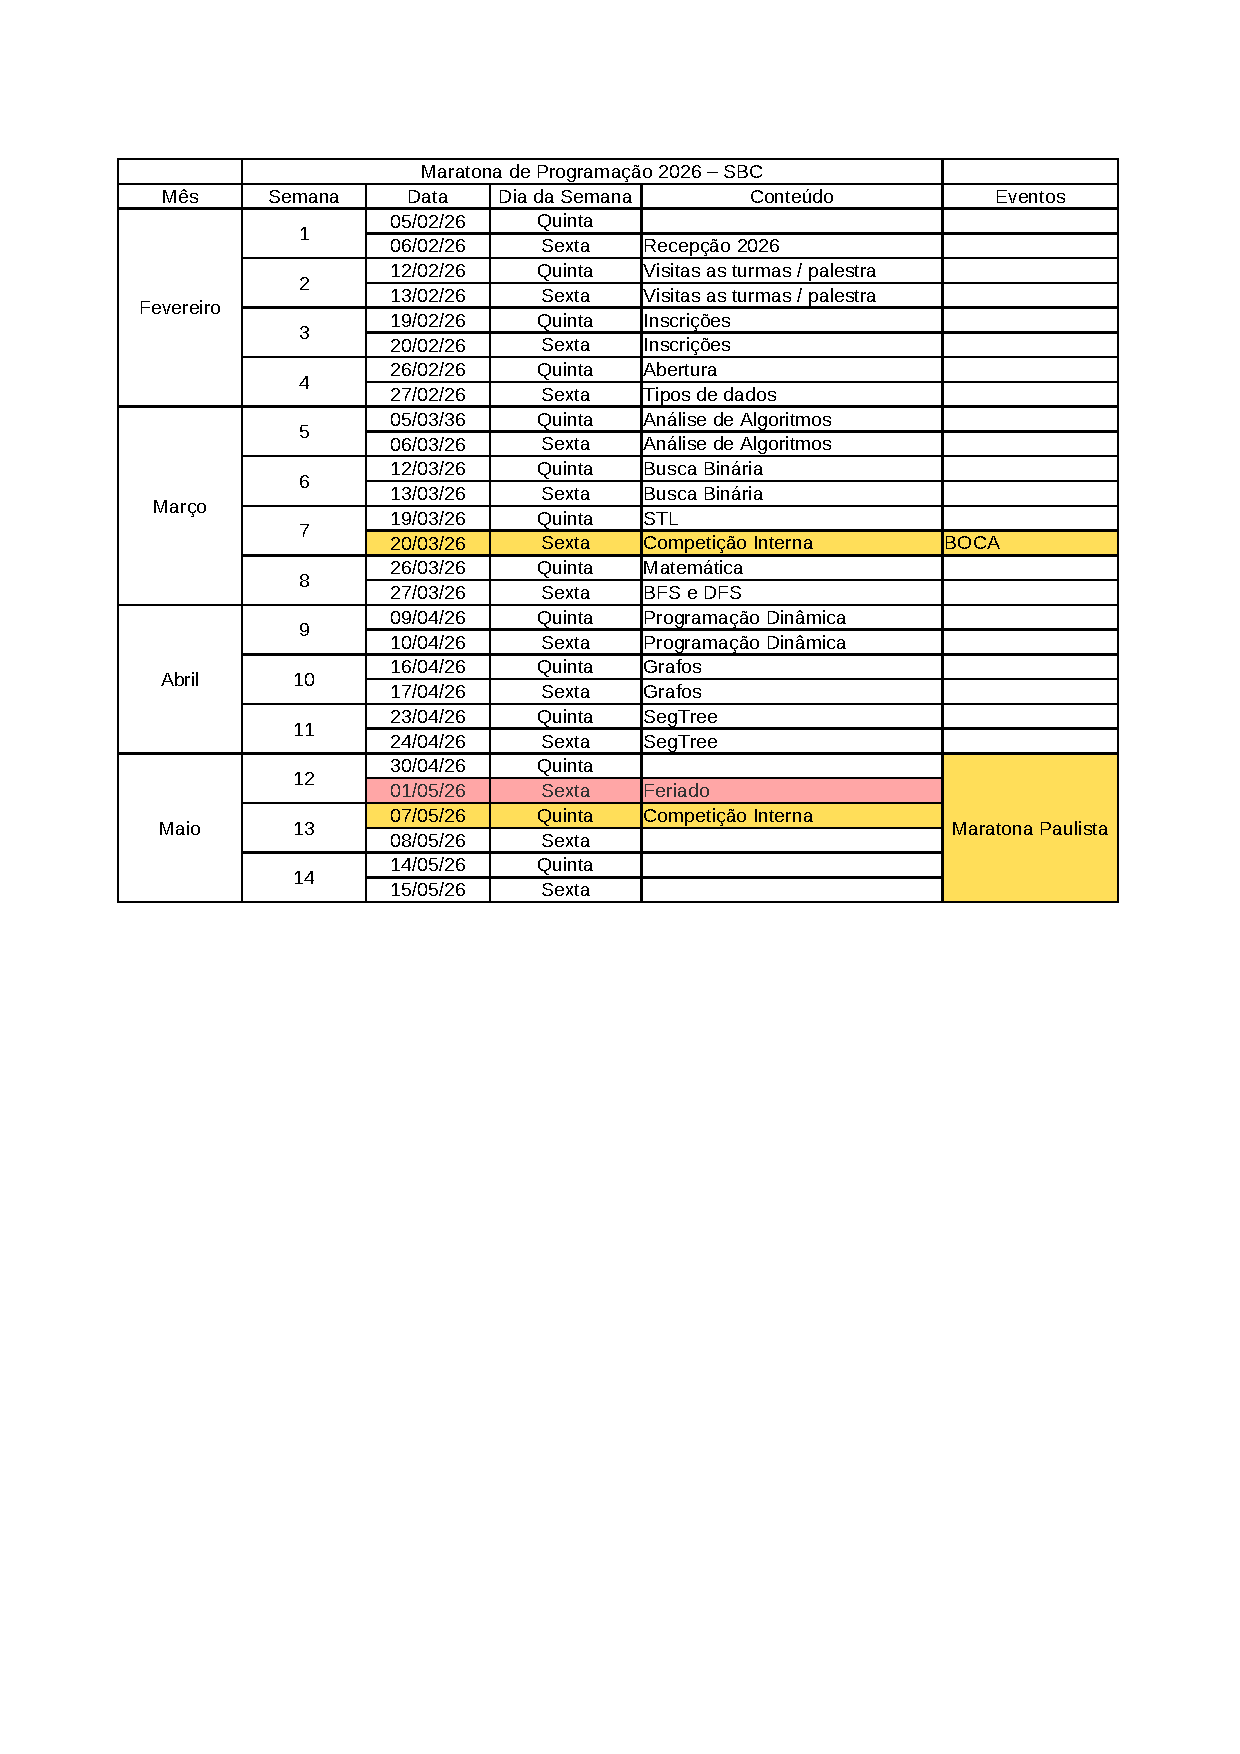
\includegraphics[scale=0.5]{cronograma-cropped.pdf}
    }\Deactivate

\end{frame}

\section{Planejamento individual de estudos}

\begin{frame}[fragile]{Planejamento}
    \textbf{Lista de exercícios para iniciantes}
    \bi%
    @ A lista atual ajuda, atrapa ou é indiferente?
    @ O que vocês acham?\pause
    \ei%
    \textbf{USACO Guide} 
\includegraphics[scale=0.3]{imagens/usaco_guide.png}
    \bi%
    @ Fazer as trilhas de estudos.
    \ei%
\end{frame}

\section{Meios de Comunicação}

\begin{frame}[fragile]{Comunicação}
    \textbf{Qual o meio de comunicação que vocês preferem?}
    \Activate\doublecolumn[0.5]{%
        \bi%
        @ e-mail
        @ Telegram
        @ What app
        \ei
    }{% ---------
        \bi
        @ Site
        @ Github
        @ Gitlab
        \ei%
    }\Deactivate
\end{frame}




\end{document}
